\documentclass{article}

% Language setting
% Replace `english' with e.g. `spanish' to change the document language
\usepackage[OT4]{fontenc}
\usepackage[polish]{babel}


% Set page size and margins
% Replace `letterpaper' with `a4paper' for UK/EU standard size
\usepackage[letterpaper,top=2cm,bottom=2cm,left=3cm,right=3cm,marginparwidth=1.75cm]{geometry}

% Useful packages
\usepackage{amsmath}
\usepackage{graphicx}
\usepackage[colorlinks=true, allcolors=blue]{hyperref}

\begin{document}

\title{%
  Separacja źródeł i transkrypcja muzyki \\ \\
  za pomocą metod sztucznej inteligencji \\
  \vspace{1em} \large Podsumowanie pracowni problemowej magisterskiej}

\author{Michał Olejnik}
\date{}
\maketitle
{
    \hypersetup{linkcolor=black}
    \tableofcontents
}

\section{Wstęp}

Celem niniejszej pracy jest przygotowanie algorytmu umożliwiającego wygenerowanie notacji muzycznej dla danego utworu. Wiele tabulatur dostępnych w sieci nie zgadza się w pełni z faktycznym utworem, a zdarza się również, że konkretny utwór ma wiele aranżacji, dla których nie są dostępny żadne notacje. Stworzenie takiego algorytmu ma na celu ułatwienie nauczenia się odgrywania konkretnej piosenki. Najbardziej istotnymi elementami utworu, na których chciałbym skupić się w tej pracy jest wokal oraz ścieżka gitarowa. Zadanie to można zrealizować wykorzystując metody separacji źródeł oraz transkrypcji muzyki.


\section{Separacja źródeł}
Zadanie separacja źródeł jest problem zdobywającym popularność w ostatnich latach. Polega ona na izolowaniu elementów składowych utworu, czyli rozdzieleniu źródeł generujących dźwięk. Różne instrumenty nagrane indywidualnie i poddane syntezie tworzą gotowy utwór. Celem separacji źródeł jest odwrócenie tego procesu. Zadanie to można podzielić na 2 kategorie: wykorzystujące falę akustyczną lub  wykorzystujące spektrogramy. Algorytmy przeprowadzające separację źródeł zazwyczaj rozpoznają 4 rodzaje komponentów składowych: głos, bas, perkusję i wszelkie inne akompaniamenty (np. gitarę, fortepian, skrzypce itd., które są grupowane razem).  \\

Wiele algorytmów przygotowanych do tego zadania bazuje na architekturze sieci U-Net \cite{ronneberger2015unet}. Jej standardowa wersja została przygotowana do segmentacji obrazów biomedycznych. Jej architektura wykorzystuje konwolucyjną sieć neuronową typu koder-dekoder, z dodatkowymi połączeniami pomiędzy odpowiadającymi sobie warstwami kodera i dekodera [Rysunek 1].\\

\begin{figure}
\centering
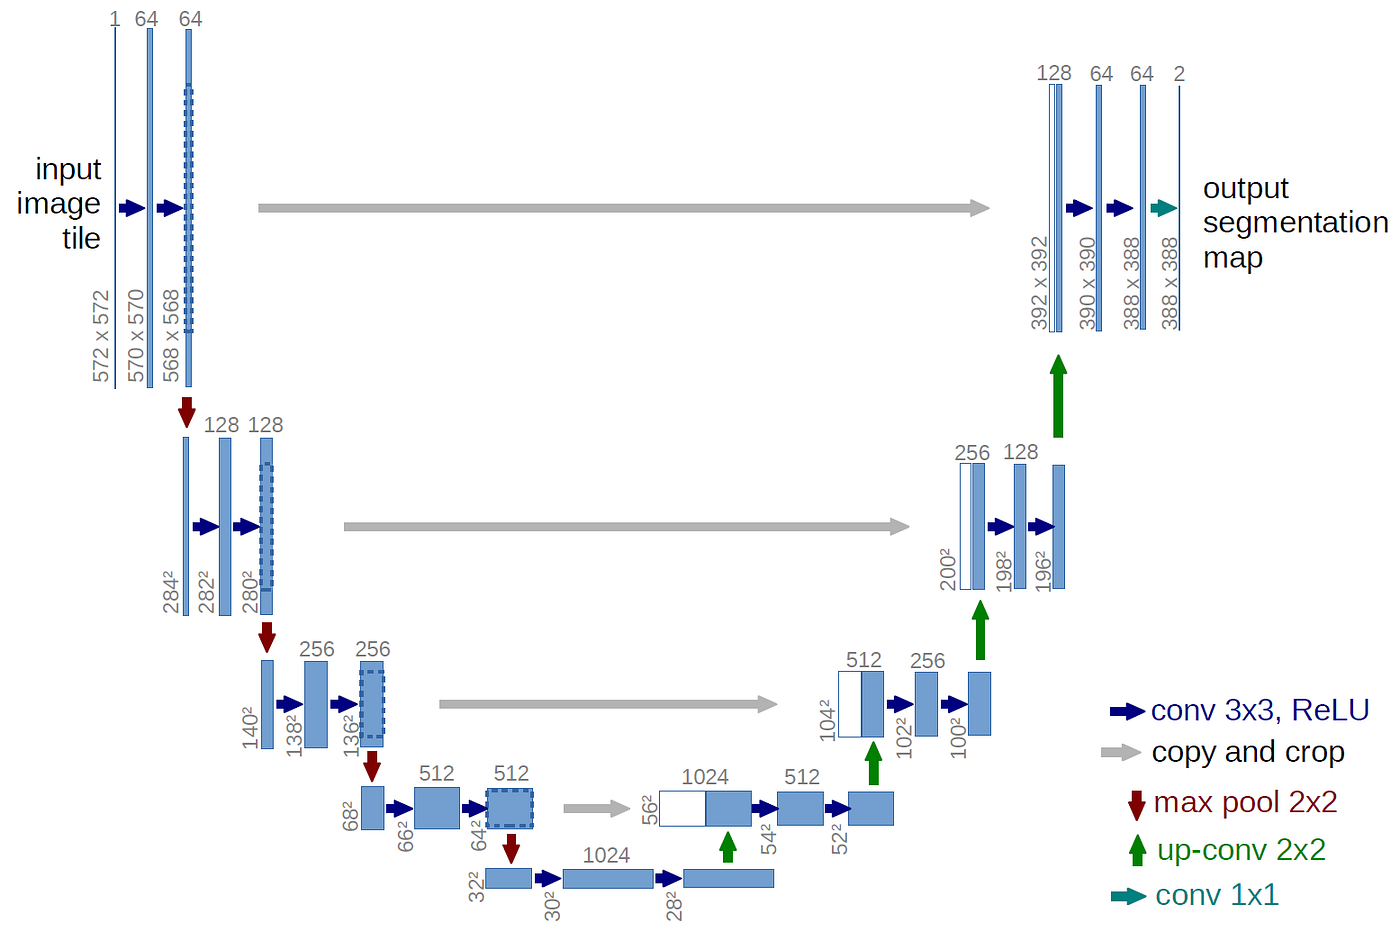
\includegraphics[width=0.75\linewidth]{unet.png}
\caption{\label{fig:unet}Schemat architektury sieci U-Net}
\end{figure}


Sieć Open-Unmix \cite{Stöter2019} jest architekturą przygotowaną do rozwiązywania problemu separacji źródeł. Sieć ta uczy się generowania spektrogramu dla konkretnego źródła, np. wokalu, na podstawie spektrogramu utworu. Wykorzystuje w tym celu trójwarstwową, dwukierunkową sieć typu LSTM [Rysunek 2.]\\

\begin{figure}
\centering
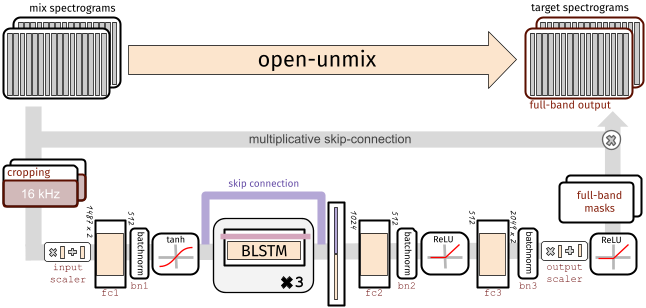
\includegraphics[width=0.75\linewidth]{open-unmix.png}
\caption{\label{fig:unet}Schemat architektury sieci Open-Unmix}
\end{figure}


Sieć Spleeter \cite{spleeter}, bazująca na wspomnianej wcześniej architekturze U-Net, jest kolejnym przykładem algorytmu rozwiązującego problem separacji źródeł. Jej architektura opiera się na sieci U-Net, z sześcioma warstwami kodera oraz sześcioma warstwami dekodera. Sieć ta została wytrenowana na wewnętrznym zbiorze danych Deezera i w odróżnieniu od poprzedniej sieci, jest w stanie rozdzielać ścieżki utworu na trzy sposoby: wokal i akompaniament, wokal, bas, perkusja i akompaniament lub wokal, bas, perkusja, pianino i akompaniament.\\


W artykule "Music Source Separation in the Waveform Domain" \cite{défossez2021music} autorzy przedstawiają architekturę Demucs działającą nie na spektrogramie, a na fali akustycznej. Architektura ta bazuje na sieci U-Net, z dodaną dwuwarstwową, dwukierunkową siecią typu LSTM pomiędzy koderem a dekoderem [Rysunek 3]. Eksperymenty przeprowadzone przez autorów wskazują, że sieć tak radzi sobie lepiej w przypadku separacji basu i perkusji, jednak podejścia korzystające ze spektrogramów, takie jak Open-Unmix czy Spleeter, radzą sobie lepiej w przypadku wokalu oraz akompaniamentu. Autorzy wskazują również na istotność augmentacji polegającej na zmianie częstotliwości i tempa oraz wykorzystaniu filtru Wienera w przetwarzaniu wyjścia sieci w przypadku sieci przyjmujących spektrogram na wejściu. \\

\begin{figure}[h!]
\centering
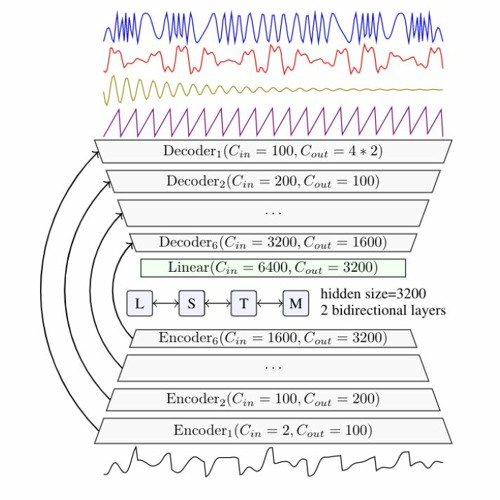
\includegraphics[width=0.75\linewidth]{demucs.jpg}
\caption{\label{fig:unet}Schemat architektury sieci Demucs}
\end{figure}


Rok po publikacji poprzedniego artykułu, został opublikowany nowy, prezentujący modyfikację sieci Demucs. Hybrid Demucs \cite{défossez2022hybrid} wykorzystuje falę akustyczną, ale również spektrogram. Umożliwia to sieci wybranie najbardziej odpowiadającej dziedziny dla konkretnego komponentu utworu. Do bazowej sieci zostały również dodane lokalna atencja oraz regularyzacja. Hybrid Demucs składa się z dwóch równoległych ścieżek, jednej odpowiadającej przetwarzaniu fali i drugiej odpowiedzialnej za przetwarzanie spektrogramu, które łączą się w ostatniej warstwie kodera [Rysunek 4.]. Na wyjściu ścieżki przetwarzającej spektrogram jest wykonywana odwrócona krótkoczasowa transformata Fouriera, w celu wygenerowania fali dźwiękowej. Fala ta jest następnie poddawana syntezie z wyjściem drugiej ścieżki. Hybrid Demucs uzyskiwał lepsze wyniki od swojego poprzednika na danych testowych. \\

\begin{figure}[h!]
\centering
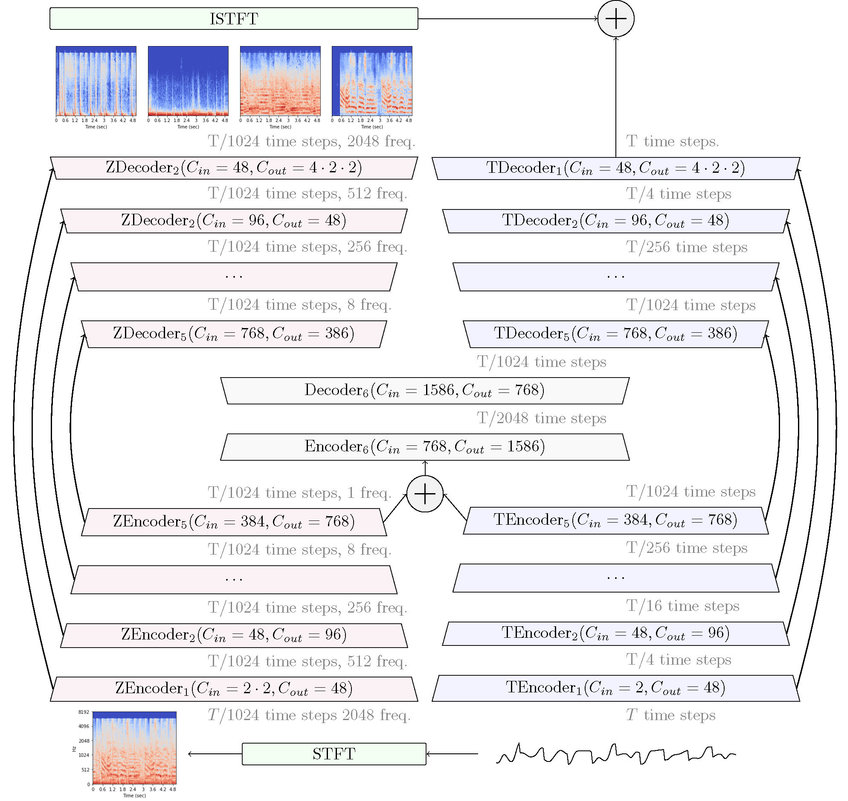
\includegraphics[width=0.75\linewidth]{hybrid_demucs.png}
\caption{\label{fig:unet}Schemat architektury sieci Hybrid Demucs}
\end{figure}


Architektura Hybrid Demucs została ponownie poddana modyfikacji. Hybrid Transformer Demucs \cite{rouard2022hybrid} zastępuje wewnętrzne warstwy pomiędzy koderem a dekoderem Transformerem, w celu wykorzystania długoczasowych zależności w utworze [Rysunek 5.]. Wewnątrz Transformera jest również użyta lokalna atencja dla każdej ze ścieżek oraz atencja krzyżowa dla ich połączenia. HT Demucs osiągał lepsze wyniki od swojego poprzednika. \\

\begin{figure}[h!]
\centering
\includegraphics[width=0.75\linewidth]{hybrid_transformer_demucs.png}
\caption{\label{fig:unet}Schemat architektury sieci Hybrid Transformer Demucs}
\end{figure}


Ciekawe podejście do zadania separacji źródeł zostało przedstawione W artykule "Score-Informed Source Separation for Musical Audio Recordings: An Overview" \cite{score-informed}. Jego autorzy wykazują użyteczność wykorzystania notacji nutowej przy wykorzystaniu algorytmu nieujemnej faktoryzacji macierzy do separacji komponentów utworu, poprzez wyrównanie w czasie notacji z odpowiadającej jej dźwiękami utworu. Podejście to nie jest jednak użyteczne w przypadku niniejszej pracy, ponieważ notacja muzyczna ma zostać wygenerowana przez algorytm i nie będzie dostępna na wejściu modelu. \\


W artykule "TOWARDS ROBUST MUSIC SOURCE SEPARATION ON LOUD COMMERCIAL MUSIC" \cite{jeon2022robust}, autorzy wskazują na istotność normalizacji głośności w zadaniu separacji źródeł. Współczesna muzyka komercyjna zazwyczaj różni się od danych, na których były uczone modele, na płaszczyźnie głośności oraz dynamiki. Jako rozwiązanie tego problemu została zaproponowana normalizacja głośności przy inferencji modelu lub wykorzystanie metody LimitAug, która dokonuje augmentacji danych. Celem metody LimitAug jest zminimalizowanie niedopasowania skali amplitudy pomiędzy danymi treningowymi, a tymi pochodzącymi ze świata. \\


\section{Automatyczna transkrypcja muzyki}
Automatyczna transkrypcja muzyki polega na konwersji sygnału akustycznego do jakiejś notacji muzycznej. Popularnymi notacjami używanymi w tym zadaniu są: notacja ABC oraz MIDI. Notacja ABC wykorzystuje litery o różnej wielkości, od a do g, do reprezentacji odpowiednich dźwięków oraz innych znaków ASCII do reprezentacji bardziej złożonych elementów. Notacja MIDI jest standardem przesyłu informacji muzycznych między urządzeniami elektronicznymi. Zawiera ona informację o wysokości dźwięku w danej chwili.\\


Transkrypcja muzyki jest problematycznym zadaniem, ze względu na potrzebę estymacji częstotliwości, estymacji głośności, rozpoznawania instrumentów, śledzenia tempa, rozpoznawania rozpoczęcia oraz zakończenia trwania konkretnych dźwięków czy kwantyzację czasu \cite{Benetos2013AutomaticMT}.\\


W artykule "Music transcription modelling and composition using deep learning" \cite{sturm2016music} zostało zaproponowane wykorzystanie sieci typu LSTM do transkrypcji muzyki do notacji ABC. Model został wyuczony na 23000 transkrypcjach, pochodzących ze zbioru zawierającego celtycką muzykę ludową.\\


W innym artykule, "Automatic Music Transcription: An Overview" \cite{Benetos2019AutomaticMT}, autorzy wskazują na kolejne problemy związane z tym zadaniem. Między innymi wspominają o ciężkich do wychwycenia zależnościach harmonicznych, różnorodności scen akustycznych, nachodzeniu na siebie instrumentów, ograniczeniach związanych z wykorzystaniem notacji zachodniej, w tym braku dobrego sposobu reprezentacji mikrotonalności, czy niewielkiej dostępności zbiorów danych dla tego zadania. \\


W 2022 roku Spotify opublikowało artykuł, w którym autorzy zaprezentowali model Notes and Multipitch, dokonujący transkrypcji muzyki do notacji MIDI \cite{bittner2022lightweight}. Model ten radzi sobie bardzo dobrze w przypadku wokalu oraz gitary. Jest to architektura konwolucyjna, generująca trzy posteriogramy na wyjściu [Rysunek 6.]. Model ten został opakowany w Pythonow'ą paczkę pod nazwą Basic Pitch. 

\begin{figure}[h!]
\centering
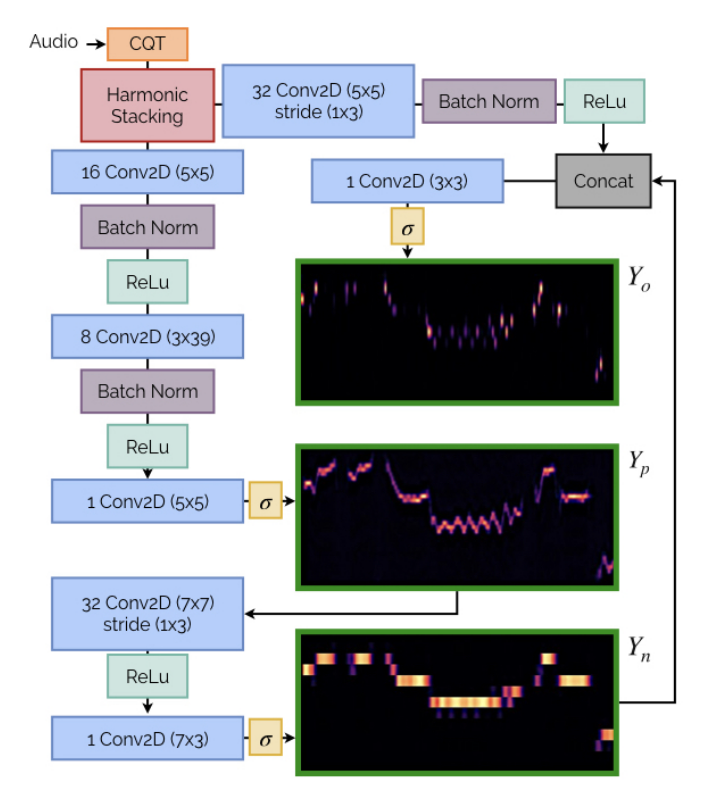
\includegraphics[width=0.75\linewidth]{notes_and_multipitch.png}
\caption{\label{fig:unet}Schemat architektury sieci Notes and Multipitch}
\end{figure}

\section{Zbiory danych}
W sieci jest dostępnych kilka zbiorów danych, których można użyć do trenowania modeli do zadań separacji źródeł oraz transkrypcji. MUSDB18 \cite{MUSDB18} jest zbiorem przygotowanym dla zadania separacji źródeł. Zawiera on 150 utworów pochodzących z różnych gatunków muzycznych. Dla każdego są dostępne ścieżki zawierające odseparowane komponenty: perkusję, bas, wokal oraz akompaniament. Moisesdb \cite{pereira2023moisesdb} jest innym datasetem dla tego zadania. Zawiera 240 utworów, pochodzących od 45 artystów, pokrywających 12 gatunków muzycznych. Ścieżki dla konkretnych komponentów są tutaj zorganizowane w dwupoziomowej hierarchii, m. in.: gitara: gitara akustyczna, gitara elektryczna, wokal: główny wokal męski, główny wokal żeński, wokal w tle itp.\\

W przypadku zadania automatycznej transkrypcji muzyki, dostępność zbiorów danych jest bardziej ograniczona. MedleyDB \cite{madleydb} zawiera 122 utwory. Może być wykorzystany do zadania separacji źródeł jak i częściowo do transkrypcji muzyki, ponieważ jego podzbiór zawiera ścieżki dla odseparowanych komponentów, ich momenty aktywacji oraz ton podstawowy. MedleyDB 2.0 \cite{Bittner2016MedleyDB2N} jest rozszerzoną wersją MedleyDB i zawiera 194 piosenki. Dodatkowo w tej wersji została również poprawiona jakość nagrań. GuitarSet \cite{guitarset} zawiera ponad trzy godziny wysokiej jakości nagrań gitar akustycznych. Zawiera informacje dotyczące tonu podstawowego oraz akordów.\\


\section{Eksperymenty}
Celem eksperymentów było sprawdzenie jak dobrze dostępne rozwiązania radzą sobie na muzyce komercyjnej. Do tego celu zostały wybrane cztery utwory muzyczne: Ren - Violet's Tale, MGMT - Little Dark Age, Metallica - Nothing Else Matters oraz Depeche Mode - Enjoy The Silence. Utwory te pochodzą z różnych gatunków muzycznych oraz zawierają różne rodzaje instrumentów. Separacja źródeł została przetestowana przy użyciu sieci Open-Unmix oraz Hybrid Demucs. Hybrid Demucs radził sobie lepiej na wymienionych utworach, co jest zgodne z wnioskami autorów tej sieci. Sieć ta jednak w przypadku niektórych piosenek generowała więcej artefaktów innych intrumentów w ścieżce basu. W przypadku obu sieci zdarzały się artefakty: wokalu w ścieżce akompaniamentu, gitary w ścieżce wokalu i perkusji w ścieżce wokalu. Hybdrid Demucs generował ścieżki w lepszej jakości niż sieć Open-Unmix. \\

Do automatycznej transkrypcji ścieżek została użyta bibilioteka basic-pitch. Wygenerowane pliki MIDI zostały zwizualizowane. Analiza wyników wskazała, że wyniki wydają się być w zadowalającym stopniu zgodne z oczekiwaniami. Nie obeszło się jednak bez artefaktów czy przycinania niektórych dzwięków [Rysunek 7.].\\

\begin{figure}[h!]
\centering
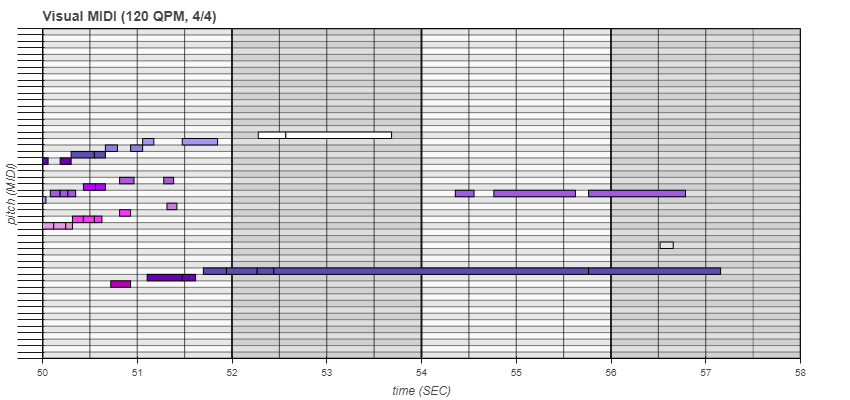
\includegraphics[width=0.75\linewidth]{bokeh_plot_guitar_ren.png}
\caption{\label{fig:unet}Wizualizacja fragmentu pliku MIDI dla ścieżki gitarowej utworu Ren - Violet's Tale}
\end{figure}

Eksperymenty sa dostępne na repozytorium GitLab \cite{repo}.


\section{Podsumowanie}
Obecnie dostępne rozwiązania są prawie wystarczające, aby stworzyć planowane przeze mnie rozwiązanie wykonujące separację źródeł oraz automatyczną transkrypcję muzyki. Problematyczne jest jedynie wygenerowanie ścieżki gitarowej, ponieważ w dostępnych modelach, należy ona do grupy akompaniamentu i w przypadku utworów które zawierają i ścieżkę gitarową i np. ścieżkę pianina, skrzypiec, saksofonu itp. ścieżka gitarowa będzie wymieszana z innymi instrumentami. Rozwiązaniem tego problemu jest stworzenie modelu, który uczyłby się generować ścieżkę gitarową równolegle z innymi i traktowałby ją jako kolejny komponent (wtedy gitara nie należałaby do grupy akompaniamentu), albo stworzenie modelu, który ze ścieżki akompaniamentu uczyłby się ekstrakcji ścieżki gitarowej. Pierwsze podejście może być problematyczne ze względu na to, że podział na wokal, bas, perkusję i akompaniament wynika z charakterystyk tych instrumentów i subiektywnej łatwości w ich odróżnieniu przez model. Drugie podejście natomiast może nie być dobre, ponieważ po separacji, ścieżki konkretnych komponentów, w tym ścieżki akompaniamentu, mogą zawierać artefakty, co może pogorszyć jakość wyekstrahowanej ścieżki gitarowej.\\

Eksperymenty pokazały dodatkowo, że jakość separacji ma duży wpływ na transkrypcję. Obecność artefaktów w konkretnych ścieżkach utrudnia poprawną transkrypcję do notacji MIDI. Oznacza to, że im lepszy model zostanie użyty do zadania separacji źródeł, tym lepsze wyniki może uzyskać model przeprowadzający autmatyczną transkrypcję muzyki.\\

Należy dodatkowo wspomnież, że notacja MIDI, może nie być odpowiednia do nauki gry konkretnego utworu i należałoby dokonać transkrypcji tej notacji do tabulatury w przypadku gitary lub do zapisu nutowego w przypadku wokalu.



\bibliographystyle{unsrt}
\bibliography{sample}

\end{document}
